\documentclass[11pt,a4paper]{amsart}
% Adapted from an OpenAI Math manuscript. See PROVENANCE.md.

\usepackage{cgeometry}
\crefname{maintheorem}{Theorem}{Theorems}
\Crefname{maintheorem}{Theorem}{Theorems}

\addbibresource{ComplexGeometry.bib}
\defbibheading{bibliography}[\refname]{\section*{#1}}
\setlength{\bibitemsep}{0pt}
\renewcommand*{\bibfont}{\footnotesize}

\allowdisplaybreaks[2]
\emergencystretch=1em

%%%%%%%%%%%%%%%%%%%%%%%%%%%%%%%%%%%%%%%%%%%%%%%%%%%%%%%%%%%%%%%%%%%%%%%%%%%%%
%% Notation
%%%%%%%%%%%%%%%%%%%%%%%%%%%%%%%%%%%%%%%%%%%%%%%%%%%%%%%%%%%%%%%%%%%%%%%%%%%%%


\usepackage{bm,xurl}
\usetikzlibrary{arrows.meta,positioning,calc}

\newcommand{\pairing}[2]{\langle #1,#2\rangle}

\title{Symplectic balls in symmetric polar products}
\author{}
\date{}

\begin{document}

\begin{abstract}
For every origin-symmetric convex body $K$ in $\mathbb{R}^n$, $n\geq2$, the Gromov width of $\operatorname{int}K\times\operatorname{int}K^\circ$ is $4$. We construct symplectic embeddings of balls of every capacity below $4$. The volume comparison gives the symmetric Mahler inequality.
\end{abstract}

\maketitle

% Adapted from an OpenAI Math manuscript. See PROVENANCE.md.
\section{Introduction}\label{sec:introduction}

Let $K\subset\mathbb{R}^n$ be an origin-symmetric convex body: a compact convex set with nonempty interior and $K=-K$. Its polar is
\[
 K^\circ=\{p\in\mathbb{R}^n:\pairing{q}{p}\le1\text{ for every }q\in K\}.
\]
We place $K$ in the position coordinates and $K^\circ$ in the conjugate momentum coordinates of $(\mathbb{R}^n_q\times\mathbb{R}^n_p,\omega_0)$, where
\[
 \omega_0=\sum_{j=1}^n dq_j\wedge dp_j,
 \qquad U_K=\operatorname{int} K\times\operatorname{int} K^\circ.
\]
For $c>0$, write
\[
 B^{2n}(c)=\{(q,p):\pi(|q|^2+|p|^2)<c\}.
\]
The Gromov width $c_G(U)$ of an open set $U\subset\mathbb{R}^{2n}$ is the supremum of the capacities $c$ for which there is a smooth embedding $e:B^{2n}(c)\to U$ satisfying $e^*\omega_0=\omega_0$.

\begin{maintheorem}\label{thm:main}
For every integer $n\ge2$ and every origin-symmetric convex body $K\subset\mathbb{R}^n$,
\[
 c_G(U_K)=4.
\]
More precisely, for every $0<c<4$ there is a smooth symplectic embedding $B^{2n}(c)\hookrightarrow U_K$.
\end{maintheorem}

This exposition follows the proof in \cite{OpenAIMathSource}.

Volume preservation gives the symmetric Mahler inequality, since $\operatorname{vol}_{2n}(B^{2n}(c))=c^n/n!$ (\cref{cor:mahler}). In dimensions $n\geq3$, the construction also transfers the ball packings of \cref{cor:polar-packings} into $U_K$.

\subsection{The ball and the polar bound}

First suppose $K$ is cut out by finitely many strip inequalities $|\langle b_j,q\rangle|\leq1$. Let $g$ be the inverse of a conformal map from the disk to a lens with tips at $\pm\ii$. For a positive integer $k$, set $f_j(z)=g(\langle b_j,z\rangle)^k$ where all linear coordinates lie in the lens. The $f_j$ have a common zero of order at least $k$ at $0$ and compact joint sublevels below $1$. The holomorphic ball construction uses a radial regularization and a compactly supported Moser deformation to embed every ball of capacity less than $\pi k$ into the joint sublevel with its K\"ahler form (\cref{sec:ball}).

A phase-space map sends the imaginary coordinate to position and integrates the K\"ahler density horizontally to obtain momentum. The planar estimate in \cref{sec:planar} bounds these horizontal integrals uniformly, including for slices approaching the lens tips. On the joint sublevel the resulting momentum belongs to $S_k\operatorname{int}K^\circ$, with $S_k/k\to\pi/4$. The map is injective by strict monotonicity in the remaining coordinate (\cref{sec:realization}). Rescaling the momentum and source ball gives capacities approaching $4$.

Approximating the polar by inner polytopes transfers the lower bound to arbitrary $K$. For the upper bound a supporting pair places $U_K$ inside a symplectic cylinder with cross-sectional area $4$, and nonsqueezing bounds its width (\cref{sec:approximation}). The supporting-slab argument is also used by Artstein-Avidan, Karasev, and Ostrover \cite[Remark~4.2]{AAKO2014}.

% Adapted from an OpenAI Math manuscript. See PROVENANCE.md.
\section{Balls from holomorphic vanishing}
\label{sec:ball}

The aim of this section is to turn the order of a holomorphic zero into the capacity of an embedded ball. We first fix the differential-form normalization, then smooth a logarithmic singularity and transport the resulting radial ball by Moser's deformation method.

Identify $\mathbb{C}^n$ with $\mathbb{R}^{2n}$ by writing $z=u+ix$.  For a smooth real function $\phi$, use the convention
\[
 \dc\phi(X)=-\frac14\,\rd \phi(\ii X),
 \qquad \ddc\phi=d(\dc\phi).
\]
In particular, the standard primitive and symplectic form are
\begin{equation}
 \lambda_0=\dc|z|^2
   =\frac12\sum_{j=1}^n(u_j\,\rd x_j-x_j\,\rd u_j),
 \qquad
 \omega_0=\ddc|z|^2=\sum_{j=1}^n du_j\wedge dx_j.
 \label{eq:ball-normalization}
\end{equation}
For every real tangent vector $X$, one has
\[
 \ddc\phi(X,iX)
 =\frac14\left.\Delta_{\zeta}\phi(z+\zeta X)\right|_{\zeta=0},
 \qquad \zeta\in\mathbb{C}.
\]
Thus a smooth function $\phi$ is plurisubharmonic precisely when these quantities are nonnegative.  In that case $\ddc(|z|^2+\phi)$ is symplectic: it is closed and its value on $(X,iX)$ is at least $|X|^2$.

We will also use that a smooth convex, coordinatewise nondecreasing function of plurisubharmonic functions is plurisubharmonic.  Indeed, on each complex line the ordinary chain rule gives
\[
 \Delta\Gamma(h_1,\ldots,h_N)
 =\sum_{j=1}^N\Gamma_j\Delta h_j
   +\sum_{i,j=1}^N\Gamma_{ij}
        \pairing{\nabla h_i}{\nabla h_j}\ge0.
\]
The first sum is nonnegative by monotonicity, and the second is nonnegative because the Hessian of $\Gamma$ is positive semidefinite.

\begin{theorem}
\label{thm:holomorphic-ball}
Let $n,m\ge1$, let $\Omega\subset\mathbb{C}^n$ be an open set containing $0$, and let $f=(f_1,\ldots,f_m):\Omega\to\mathbb{C}^m$ be holomorphic.  Suppose that, for some integer $k\ge1$,
\begin{enumerate}[label=\textup{(\roman*)}]
 \item $f^{-1}(0)=\{0\}$ and $|f(z)|=O(|z|^k)$ as $z\to0$;
 \item for every $0<s<1$, the set
 $\{z\in\Omega:|f(z)|^2\le s\}$ is a compact subset of $\Omega$.
\end{enumerate}
Set
\[
 \tau=|f|^2,\qquad V=\{z\in\Omega:\tau(z)<1\},
 \qquad \omega=\ddc(|z|^2+\tau).
\]
For every $0<c<\pi k$, there is a smooth symplectic embedding
\[
 \bigl(B^{2n}(c),\omega_0\bigr)\longrightarrow(V,\omega).
\]
\end{theorem}

\begin{proof}
\noindent\emph{A logarithmic potential.} For a holomorphic tuple, differentiation along a complex line gives
\begin{align}
 \ddc\tau(X,iX)&=|df(X)|^2,\notag\\
 \ddc\log\tau(X,iX)
 &=\frac{|f|^2|df(X)|^2
       -\left|\sum_{j=1}^m\overline{f_j}\,\rd f_j(X)\right|^2}{|f|^4}
 \quad\text{on }\Omega\setminus\{0\}.
 \label{eq:ball-log-levi}
\end{align}
The second expression is nonnegative by Cauchy--Schwarz.  Hence $\tau$ and, away from its zero, $\log\tau$ are plurisubharmonic.

Fix $0<a<k$; we will embed the ball of capacity $\pi a$.  Choose
\[
 \frac ak<b<1,\qquad a<\mu<bk.
\]
Choose numbers $\log b<t_-<t_+<0$ and a smooth nondecreasing cutoff $\beta:\mathbb{R}\to[0,1]$ which is $0$ for $t\le t_-$ and $1$ for $t\ge t_+$. Define $\chi$ on $(-\infty,0)$ by
\[
 \chi'(t)=b+\beta(t)(\ee^t-b),
\]
choosing its additive constant so that $\chi(t)=\ee^t$ for $t\ge t_+$. This is possible since $\chi'=\ee^t$ there.  Moreover, $\chi'>0$ and
\[
 \chi''(t)=\beta'(t)(\ee^t-b)+\beta(t)\ee^t\ge0,
\]
because the transition occurs where $\ee^t>b$.  For $t\le t_-$, the function $\chi$ is affine with slope $b$.

It follows that
\[
 H=\chi(\log\tau)
\]
is smooth and plurisubharmonic on $V\setminus\{0\}$ and satisfies $H=\tau$ wherever $\tau\ge s_0:=\ee^{t_+}$.  The vanishing assumption gives $\tau(z)\le C_0|z|^{2k}$ near zero.  Since $\chi$ is eventually affine, there is a constant $C_1$ such that
\begin{equation}
 H(z)\le bk\log|z|^2+C_1
 \quad\text{for all sufficiently small }z\ne0.
 \label{eq:ball-singularity}
\end{equation}

\smallskip
\noindent\emph{Smoothing near the origin.} The strict inequality $\mu<bk$ lets a smooth radial logarithm dominate $H$ close to zero while remaining below it on an outer sphere. Write $B_r=\{z\in\mathbb{C}^n:|z|<r\}$, and choose $r_2>0$ with $\overline{B}_{r_2}\subset V$.  For $0<\delta\le1$, consider
\[
 P_\delta(z)=\mu\log(|z|^2+\delta)-M.
\]
For each fixed $r>0$, the radial calculation below identifies $(B_r,\ddc(|z|^2+P_\delta))$ with a standard ball whose squared radius is $r^2+\mu r^2/(r^2+\delta)$. Since $\mu>a$, this exceeds $a$ for all sufficiently small $\delta$. We will therefore arrange that the modified potential agrees with $P_\delta$ on a ball whose radius is fixed before $\delta$ is chosen.

The functions $P_\delta$ are plurisubharmonic by \eqref{eq:ball-log-levi}, applied to the nowhere-zero holomorphic tuple $(\sqrt\delta,z_1,\ldots,z_n)$.  Choose $M$ so that
\[
 M>\mu\log(r_2^2+1)-\min_{|z|=r_2}H(z)+2.
\]
The minimum is finite because $f$ has no zero on this sphere.  Then $P_\delta<H-2$ on $|z|=r_2$ for every $0<\delta\le1$. On the other hand, \eqref{eq:ball-singularity} gives
\[
 P_\delta(z)-H(z)
 \ge(\mu-bk)\log|z|^2-M-C_1.
\]
As $z\to0$, this lower bound tends to $+\infty$, uniformly in $\delta$. We may therefore fix $0<r_1<r_2$, independently of $\delta$, such that
\begin{equation}
 P_\delta>H+2\quad\text{on }0<|z|\le r_1
 \quad\text{for every }0<\delta\le1.
 \label{eq:ball-inner-domination}
\end{equation}
Fix from now on one positive $\delta$ satisfying
\begin{equation}
 0<\delta<\min\left\{1,\ r_1^2\left(\frac\mu a-1\right)\right\}.
 \label{eq:ball-delta-choice}
\end{equation}
The upper bound is positive because $\mu>a$.

We next replace the singularity of $H$ by $P_\delta$ using a regularized maximum, the standard gluing device in Richberg's smoothing method; see \cite[Section~2]{HarveyLawsonPlis2020}. A related replacement of K\"ahler potentials appears in \cite[Proposition~3.3]{WittNystrom2018} in a projective setting. We give the elementary two-function construction explicitly. Let $\vartheta\in C_c^\infty((-1,1))$ be nonnegative and even, with $\int_{\mathbb{R}}\vartheta=1$, and set
\[
 \rho(s)=\int_{\mathbb{R}}|s-t|\vartheta(t)\,\rd t,
 \qquad
 \operatorname{rmax}(h,p)=\frac{h+p+\rho(h-p)}2.
\]
The function $\rho$ is smooth and convex, with $|\rho'|\le1$, and equals $|s|$ for $|s|\ge1$.  Thus $\operatorname{rmax}$ is smooth, convex, nondecreasing in both arguments, and equals $\max(h,p)$ when $|h-p|\ge1$.  Define $\widetilde H$ to be $\operatorname{rmax}(H,P_\delta)$ on $B_{r_2}\setminus\{0\}$, to be $H$ outside $B_{r_2}$, and to take the value $P_\delta(0)$ at zero. The outer comparison gives equality with $H$ in a neighborhood of $\partial B_{r_2}$, and \eqref{eq:ball-inner-domination} gives equality with $P_\delta$ on $B_{r_1}$.  Consequently $\widetilde H$ is smooth and plurisubharmonic on all of $V$.

The difference $\widetilde H-\tau$ has compact support in $V$. Indeed, set $s_2=\max_{\overline B_{r_2}}\tau<1$, choose $\max(s_0,s_2)<\sigma<1$, and put
\begin{equation}
 C=\{z\in\Omega:\tau(z)\le\sigma\}.
 \label{eq:ball-support}
\end{equation}
This is a compact subset of $V$ by hypothesis.  Outside $C$ a point lies outside $\overline B_{r_2}$ and has $H=\tau$, so that $\widetilde H-\tau$ vanishes there.

\smallskip
\noindent\emph{Moser's deformation.} The support estimate gives a complete flow for Moser's deformation \cite[Section~4]{Moser1965}. Use the symplectic forms
\[
 \omega_s=\ddc\bigl(|z|^2+(1-s)\tau+s\widetilde H\bigr),
 \qquad 0\le s\le1,
\]
and write $\widetilde\omega=\omega_1$.  Each form is symplectic because the two non-Euclidean potentials are plurisubharmonic.  Define the smooth time-dependent vector field $Y_s$ by
\[
 \iota_{Y_s}\omega_s=-\gamma,
 \qquad \gamma=\dc(\widetilde H-\tau).
\]
Both $\gamma$ and every $Y_s$ are supported in the fixed compact set $C$.  Extending $Y_s$ by zero outside $V$ gives a smooth vector field on $\mathbb{C}^n$, with its coefficients and first derivatives bounded uniformly for $s\in[0,1]$.  The ordinary differential equation for this field has a flow $\varphi_s$ throughout this time interval. The ambient flow fixes $\mathbb{C}^n\setminus V$ pointwise and hence restricts to diffeomorphisms of $V$.  This argument applies even if $V$ is disconnected and places no regularity assumption on its boundary.

Since $d\omega_s=0$, differentiation of pullbacks gives
\[
 \frac{d}{ds}\varphi_s^*\omega_s
 =\varphi_s^*\bigl(d\gamma+d\iota_{Y_s}\omega_s\bigr)=0.
\]
Therefore
\begin{equation}
 \varphi_1^*\widetilde\omega=\omega,
 \qquad
 \varphi_1^{-1}:(V,\widetilde\omega)\longrightarrow(V,\omega)
 \text{ is symplectic}.
 \label{eq:ball-moser}
\end{equation}

\smallskip
\noindent\emph{The ball in the radial metric.} The deformation has reduced the problem to an explicit radial form. On $B_{r_1}$ the new potential, up to the additive constant $-M$, is $\Psi(|z|^2)$, where
\[
 \Psi(t)=t+\mu\log(t+\delta).
\]
Define the radial map
\[
 R(z)=\sqrt{\Psi'(|z|^2)}\,z
     =\sqrt{1+\frac\mu{|z|^2+\delta}}\,z.
\]
This is the radial case of the symplectic-coordinate construction in \cite[proof of Theorem~1.1, Equation~(23)]{LoiZuddas2008}. In the pullback of $\lambda_0$ from \eqref{eq:ball-normalization}, the terms differentiating the radial factor cancel.  Hence
\[
 R^*\lambda_0=\Psi'(|z|^2)\lambda_0=\dc\Psi(|z|^2),
 \qquad R^*\omega_0=\widetilde\omega\big|_{B_{r_1}}.
\]
The squared radial coordinate is strictly increasing, because
\[
 \frac{d}{dt}\bigl(t\Psi'(t)\bigr)
 =\frac{d}{dt}\left(t+\frac{\mu t}{t+\delta}\right)
 =1+\frac{\mu\delta}{(t+\delta)^2}>0.
\]
At zero the map is smooth and has derivative $DR(0)=\sqrt{1+\mu/\delta}\,I$, so its inverse is smooth there as well.  Thus $R$ is a diffeomorphism from $B_{r_1}$ onto the standard ball $B^{2n}(\pi Q_\delta)$, where
\[
 Q_\delta=r_1^2+\frac{\mu r_1^2}{r_1^2+\delta}>a
\]
by \eqref{eq:ball-delta-choice}.  If $\iota:B_{r_1}\hookrightarrow V$ denotes inclusion, the map
\[
 \varphi_1^{-1}\circ\iota\circ
       R^{-1}\big|_{B^{2n}(\pi a)}:
 B^{2n}(\pi a)\longrightarrow V
\]
is a smooth embedding, and its pullback of $\omega$ is $\omega_0$ by \eqref{eq:ball-moser} and the radial pullback identity. Since $a$ was arbitrary in $(0,k)$, the theorem follows.
\end{proof}

% Adapted from an OpenAI Math manuscript. See PROVENANCE.md.
\section{A planar coordinate and a uniform slice estimate}
\label{sec:planar}

We use Gross's conformal map $\psi$ for the uniform distribution \cite[Section~3.2]{Gross2019}, with the rotation $F(w)=i\psi(iw)$. There is no scaling. The same lens appears in \cite[Section~3]{SymmetricCompanion2026}; its half-width $\lambda(t)$ is the function $V(t)$ used here. We establish its needed properties directly and then prove a uniform slice estimate that controls the momentum coordinates in the polar product.

\begin{lemma}\label{lem:planar-map}
The holomorphic function
\begin{equation}\label{eq:planar-F}
 F(w)=\frac{8}{\pi^2}\sum_{\ell=0}^{\infty}
       \frac{(-1)^\ell w^{2\ell+1}}{(2\ell+1)^2},
 \qquad w\in\mathbb{D},
\end{equation}
is a biholomorphism from $\mathbb{D}$ onto a bounded domain $D$. It is odd, commutes with conjugation, and satisfies $F(0)=0$. The imaginary coordinates of $D$ range over $(-1,1)$, and for each $t\in(-1,1)$ there is a finite $V(t)>0$ such that
\begin{equation}\label{eq:horizontal-slices}
 \{v\in\mathbb{R}:v+it\in D\}=(-V(t),V(t)).
\end{equation}
Write $F(ir)=iT(r)$ for $0\le r<1$.  The function $T$ increases strictly from $0$ to $1$, with
\begin{equation}\label{eq:planar-T}
 T'(r)=\frac{8}{\pi^2}\frac{\operatorname{arctanh}r}{r}
 \quad(0<r<1),
 \qquad \lim_{r\uparrow1}T'(r)=+\infty.
\end{equation}
For fixed $t\in(-1,1)$, put $r_0=T^{-1}(|t|)$.  The positive horizontal slice is parametrized by
\[
 w(r,t)=re^{i\theta(r,t)},\qquad
 F(w(r,t))=v(r,t)+it,\qquad r_0<r<1,
\]
where $-\pi/2<\theta(r,t)<\pi/2$ and $v(r,t)$ increases strictly from $0$ to $V(t)$.
\end{lemma}

\begin{proof}
\noindent\textit{The map and its angular derivative.} The series in \eqref{eq:planar-F} is absolutely summable on the closed disk.  Hence $F$ is bounded, odd, and commutes with conjugation. Termwise differentiation in the open disk gives
\begin{equation}\label{eq:planar-arctan}
 wF'(w)=\frac{8}{\pi^2}\arctan w,
 \qquad
 \arctan w=\frac{1}{2i}\log\frac{1+iw}{1-iw}.
\end{equation}
Here the logarithm is the branch on the right half-plane that is real on the positive real axis.  Indeed,
\[
 \Re\frac{1+iw}{1-iw}
   =\frac{1-|w|^2}{|1-iw|^2}>0
 \qquad (w\in\mathbb{D}).
\]
This also shows that $\arctan w=0$ only at $w=0$. Thus $F'$ has no zeros away from the origin, and the series gives $F'(0)=8/\pi^2\ne0$.

For $w=re^{i\theta}$, define
\begin{equation}\label{eq:planar-A}
 A(r,\theta)=\Re\bigl(wF'(w)\bigr)
   =\frac{4}{\pi^2}
       \arctan\frac{2r\cos\theta}{1-r^2}.
\end{equation}
To obtain the last identity, the imaginary part of the fraction in \eqref{eq:planar-arctan}, divided by its real part, is $2r\cos\theta/(1-r^2)$, and its argument lies in $(-\pi/2,\pi/2)$.  On the right semicircle, $0<A(r,\theta)<2/\pi$.  The identities
\begin{equation}\label{eq:planar-polar-derivatives}
 \partial_r F(re^{i\theta})=\frac{wF'(w)}{r},
 \qquad
 \partial_\theta F(re^{i\theta})=iwF'(w)
\end{equation}
therefore show that $\Re F(w)>0$ in the right half-disk: its radial derivative is positive, and its value tends to zero at the origin. They also show that $\Im F(re^{i\theta})$ increases strictly with $\theta$ on each right semicircle.

Oddness and conjugation symmetry give $F(ir)=iT(r)$ with real $T$. Since $T'(r)=F'(\ii r)$ and $\arctan(\ii r)=\ii\operatorname{arctanh}r$, \eqref{eq:planar-arctan} gives \eqref{eq:planar-T}.  In particular, $T$ is strictly increasing, $T(0)=0$, and $T'(r)$ diverges as $r\uparrow1$. Since $F(r)$ is real, \eqref{eq:planar-polar-derivatives} also gives
\[
 T(r)=\int_0^{\pi/2}A(r,\theta)\,\rd \theta.
\]
The integrand is bounded by $2/\pi$ and tends to $2/\pi$ at every $\theta\in[0,\pi/2)$ as $r\uparrow1$.  Dominated convergence therefore gives $T(r)\to1$.

\medskip \noindent\textit{Horizontal slices and global invertibility.} Fix $|t|<1$ and let $T(r_0)=|t|$.  For every $r\in(r_0,1)$, the strictly increasing imaginary coordinate on the right semicircle ranges from $-T(r)$ to $T(r)$.  There is consequently exactly one angle $\theta(r,t)$ there with imaginary coordinate $t$. It depends smoothly on $r$, since its angular derivative is $A>0$. Writing $wF'(w)=A+iB$, implicit differentiation at fixed $t$ gives
\[
 \partial_r\theta=-\frac{B}{rA},
 \qquad
 \partial_r v=\frac{A}{r}-B\,\partial_r\theta
             =\frac{A^2+B^2}{rA}.
\]
Thus
\begin{equation}\label{eq:horizontal-radius-derivative}
 \frac{\partial v}{\partial r}(r,t)
   =\frac{|wF'(w)|^2}{rA(r,\theta(r,t))}>0.
\end{equation}
As $r\downarrow r_0>0$, the angle tends to the appropriate imaginary-axis endpoint of the semicircle, so $v(r,t)\to0$.  If $r_0=0$, the same limit follows from $F(0)=0$.  Boundedness of $F$ now shows that $v(r,t)$ maps $(r_0,1)$ continuously and strictly increasingly onto an interval $(0,V(t))$, where $0<V(t)<\infty$.

This parametrization proves injectivity on each positive horizontal slice.  The reflection identity $F(-\overline w)=-\overline{F(w)}$ gives the negative slices, and the strict monotonicity of $T$ gives injectivity on the imaginary axis. The right half-disk, imaginary axis, and left half-disk have images with positive, zero, and negative real parts, respectively.  Hence $F$ is globally injective.  Every point of its image has imaginary coordinate in $(-1,1)$, and every such coordinate occurs on the imaginary axis. This proves \eqref{eq:horizontal-slices}.  Since $F'\ne0$, the local holomorphic inverses combine into a holomorphic inverse $g:D\to\mathbb{D}$.
\end{proof}

\Cref{fig:lens-slices} illustrates the radial parametrization of a horizontal slice.  Along the right half of the highlighted disk curve, $\Im F(w)=t$ stays fixed while $|w|$ increases, and its image moves to the right along the horizontal slice. Equation~\eqref{eq:horizontal-radius-derivative} therefore allows us to rewrite horizontal integrals using the disk radius $r$, as we do below.
% Adapted from an OpenAI Math manuscript. See PROVENANCE.md.
\begin{figure}[htb]
  \centering
  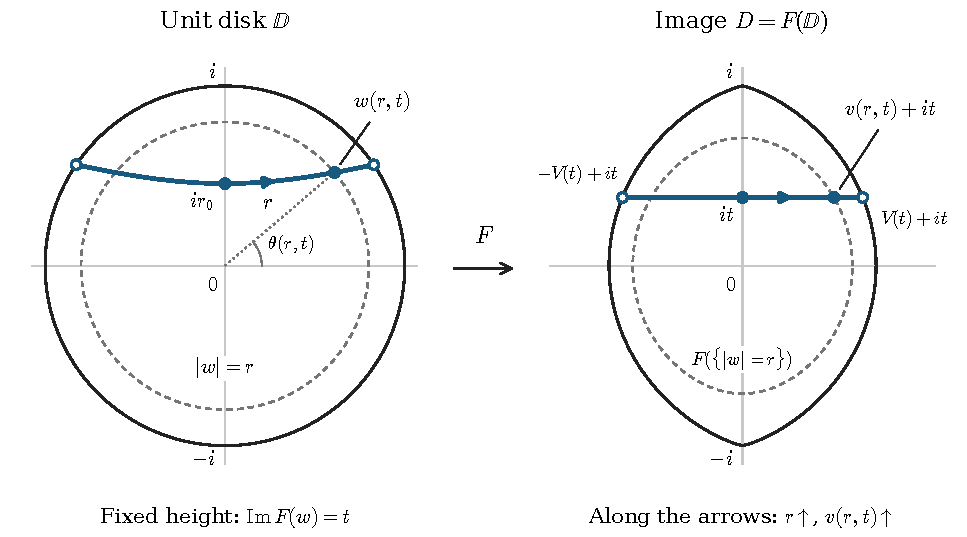
\includegraphics[width=\linewidth]{figures/lens-slices.pdf}
  \caption{A fixed horizontal slice and its preimage, illustrated for $t>0$.
  Along the right half of the highlighted preimage curve in the left panel,
  $r$ increases from
  $r_0=T^{-1}(t)$ to $1$, while $v(r,t)$ increases from $0$ to $V(t)$.
  The dashed circle and its image pass through the corresponding marked
  points. Open markers indicate boundary limits.}
  \label{fig:lens-slices}
\end{figure}


For an integer $k\ge2$, define the signed slice integral
\begin{equation}\label{eq:slice-primitive}
 J_k(v,t)=k^2\int_0^v
       |g(h+it)|^{2k-2}|g'(h+it)|^2\,\rd h,
 \qquad v+it\in D.
\end{equation}
The segment of integration lies in $D$ by \cref{lem:planar-map}.

\begin{proposition}\label{prop:uniform-slice}
Each $J_k$ is smooth on $D$, is odd in $v$, and satisfies
\begin{equation}\label{eq:slice-derivative}
 \partial_v J_k(v,t)
    =k^2|g(v+it)|^{2k-2}|g'(v+it)|^2\ge0.
\end{equation}
There is a sequence $\epsilon_k\ge0$, depending only on $F$, with $\epsilon_k\to0$ such that, simultaneously for every $v+it\in D$,
\begin{equation}\label{eq:uniform-slice}
 \frac{|J_k(v,t)|}{k}
    \le\frac{\pi}{4}|g(v+it)|^{2k}+\epsilon_k.
\end{equation}
\end{proposition}

\begin{proof}
\noindent\emph{The disk radius as a variable.} For any fixed $v+it\in D$, the horizontal segment from $it$ to $v+it$ is a compact subset of the open set $D$; the same is true for all sufficiently nearby endpoints and heights.  The formula
\[
 J_k(v,t)=k^2v\int_0^1
       |g(av+it)|^{2k-2}|g'(av+it)|^2\,\rd a
\]
then proves smoothness by differentiation under the integral. The integrand is smooth even at the zero of $g$, since $|g|^{2k-2}=(|g|^2)^{k-1}$ and $k$ is an integer. Equation~\eqref{eq:slice-derivative} follows from the fundamental theorem of calculus.  The symmetry $g(-\overline\zeta)=-\overline{g(\zeta)}$ makes the density in \eqref{eq:slice-primitive} even in its real coordinate.  Thus $J_k(-v,t)=-J_k(v,t)$, and it suffices to estimate $v>0$.

Fix such a point and put
\[
 R=|g(v+it)|,\qquad r_0=T^{-1}(|t|).
\]
Along its positive horizontal slice, the radius increases from $r_0$ to $R$.  Since $g'(F(w))=1/F'(w)$, \eqref{eq:horizontal-radius-derivative} gives
\begin{equation}\label{eq:slice-radial-integral}
 \frac{J_k(v,t)}{k}
    =k\int_{r_0}^{R}
       \frac{r^{2k-1}}{A(r,\theta(r,t))}\,\rd r.
\end{equation}
Indeed, $|g'|^2\,\rd v=(r/A)\,\rd r$. At the lower endpoint this is understood as an improper integral: perform the change of variables first on a segment beginning at a positive real coordinate, and then let that coordinate decrease to zero. The original integrand is smooth on the full compact segment, so its integral is finite; the nonnegative transformed integrals converge to the same value.  This argument also covers $t=0$, when $r_0=0$.

The leading constant comes from splitting $1/A$ into $\pi/2$ and the nonnegative excess $1/A-\pi/2$, since $0<A<2/\pi$. The constant part in \eqref{eq:slice-radial-integral} contributes $\frac{\pi}{4}(R^{2k}-r_0^{2k})$.  It therefore suffices to bound the remaining weighted integral uniformly over all heights and endpoints by a quantity tending to zero as $k\to\infty$.

\smallskip
\noindent\emph{The estimate at the tips.} The denominator can be small near the ends of the right semicircle. Suppose $1/2\le r<1$ and set
\[
 s=\frac{\pi}{2}-|\theta|\in(0,\pi/2],
 \qquad
 X=\frac{2r\sin s}{1-r^2}.
\]
For every $X>0$,
\begin{equation}\label{eq:reciprocal-arctan}
 \frac{1}{\arctan X}-\frac{2}{\pi}\le\frac{2}{X}.
\end{equation}
For $X\le1$, this follows from $\arctan X\ge X/2$; for $X\ge1$, use $\pi/2-\arctan X=\arctan(1/X)\le1/X$ and $\arctan X\ge\pi/4$.  Combining \eqref{eq:reciprocal-arctan} with $\sin s\ge2s/\pi$ and $(1+r)/(2r)\le3/2$, we obtain
\begin{equation}\label{eq:A-angular-bound}
 \frac1{A(r,\theta)}
    \le\frac{\pi}{2}+\frac{3\pi^3}{8}\frac{1-r}{s}.
\end{equation}
On the other hand, the vertical gap to the semicircle endpoint is
\begin{align}
 \Delta(r,\theta)
   &:=T(r)-|\Im F(re^{i\theta})|
     =\int_0^s\frac{4}{\pi^2}
          \arctan\frac{2r\sin\xi}{1-r^2}\,d\xi \notag\\
   &\le\frac{4r}{\pi^2(1-r^2)}s^2
     \le\frac{2}{\pi^2}\frac{s^2}{1-r}.
 \label{eq:vertical-gap}
\end{align}
Here we used $\arctan y\le y$ and $\sin\xi\le\xi$. The last inequality supplies the lower bound $s\ge(\pi/\sqrt2)\sqrt{\Delta(r,\theta)(1-r)}$. Consequently, with the absolute constant $C_0=3\sqrt2\pi^2/8$, \eqref{eq:A-angular-bound} implies
\begin{equation}\label{eq:A-slice-bound}
 \frac1{A(r,\theta(r,t))}
   \le\frac{\pi}{2}
        +C_0\sqrt{\frac{1-r}{T(r)-|t|}}
 \qquad (r\ge1/2,\ r>r_0).
\end{equation}

\smallskip
\noindent\emph{The compact part of the integral.} Fix a radius $r_*\in(1/2,1)$.  The part of the original horizontal integral for which $|g|\le r_*$ is uniformly bounded, after division by $k$, by
\begin{equation}\label{eq:slice-inner-bound}
 C_*k r_*^{2k-2},
 \qquad
 C_*:=\operatorname{diam}(D)
          \max_{|w|\le r_*}|F'(w)|^{-2}<\infty.
\end{equation}
To see this, the radius is strictly increasing along the positive slice, so the relevant portion is exactly its initial segment ending at radius $\min(R,r_*)$, when $r_0\le r_*$, and is empty otherwise. Every point of this segment lies in $F(\{|w|\le r_*\})$, and its horizontal length is at most $\operatorname{diam}(D)$. This includes the case $R\le r_*$, when it is the whole integral.

If an outer portion remains, put
\[
 r_a=\max(r_0,r_*),\qquad
 L_*:=\inf_{r_*\le r<1}T'(r)>0.
\]
Since $T(r_a)\ge T(r_0)=|t|$, for $r>r_a$ we have
\begin{equation}\label{eq:gap-tail-bound}
 T(r)-|t|\ge T(r)-T(r_a)\ge L_*(r-r_a).
\end{equation}
\eqref{eq:slice-radial-integral} and \eqref{eq:A-slice-bound} therefore bound the outer contribution by
\begin{equation}\label{eq:slice-outer-bound}
 \frac{\pi}{4}\bigl(R^{2k}-r_a^{2k}\bigr)
  +\frac{C_0}{\sqrt{L_*}}\,
       k\int_{r_a}^{1}r^{2k-1}
                 \sqrt{\frac{1-r}{r-r_a}}\,\rd r.
\end{equation}
The extension of the error integral from $R$ to $1$ uses its nonnegativity and removes any dependence on the distance $R-r_a$.

The last integral has an absolute bound, including when its lower endpoint depends on $k$.  Write
\[
 I(k,r_a)=k\int_{r_a}^{1}r^{2k-1}
                    \sqrt{\frac{1-r}{r-r_a}}\,\rd r,
 \qquad H=k(1-r_a).
\]
The substitution $y=k(1-r)$ gives
\begin{align*}
 I(k,r_a)
   &=\int_0^H(1-y/k)^{2k-1}\sqrt{\frac{y}{H-y}}\,\rd y\\
   &\le\int_0^H \ee^{-y}\sqrt{\frac{y}{H-y}}\,\rd y,
\end{align*}
since $\log r\le-(1-r)$ and $2k-1\ge k$. On $[0,H/2]$ the square-root factor is at most one.  On $[H/2,H]$, bound the exponential by $\ee^{-H/2}$ and use
\[
 \int_0^H\sqrt{\frac{y}{H-y}}\,\rd y=\frac{\pi H}{2}.
\]
It follows that
\begin{equation}\label{eq:uniform-endpoint-integral}
 I(k,r_a)\le 1+\frac{\pi H}{2}\ee^{-H/2}
           \le 1+\frac{\pi}{e}.
\end{equation}
The same integral without its exponential factor also gives $I(k,r_a)\le\pi H/2$.  These estimates hold for every $H>0$, covering both $H\downarrow0$ and $H\to\infty$.

Combining \eqref{eq:slice-inner-bound}, \eqref{eq:slice-outer-bound}, and \eqref{eq:uniform-endpoint-integral}, and using symmetry when $v<0$, we have, for every $v+it\in D$,
\begin{equation}\label{eq:slice-uniform-error-bound}
 \frac{|J_k(v,t)|}{k}-\frac{\pi}{4}|g(v+it)|^{2k}
   \le C_*k r_*^{2k-2}
          +\frac{C_0(1+\pi/e)}{\sqrt{L_*}}.
\end{equation}
When there is no outer portion, the first term alone bounds the excess, so the same displayed inequality remains valid.  It is also valid at $v=0$.

\smallskip
\noindent\emph{The uniform error.} The cutoff radius will be chosen before the power $k$, so the estimates above allow the slice height and both radial endpoints to move with $k$. Define explicitly
\begin{equation}\label{eq:slice-error-sequence}
 \epsilon_k=
 \max\left\{0,\ \sup_{v+it\in D}
     \left(\frac{|J_k(v,t)|}{k}
                  -\frac{\pi}{4}|g(v+it)|^{2k}\right)\right\}.
\end{equation}
\eqref{eq:slice-uniform-error-bound} makes this supremum finite for each $k$.  For fixed $r_*$, its first error term tends to zero as $k\to\infty$.  Moreover, \eqref{eq:planar-T} gives
\[
 L_*\ge\frac{8}{\pi^2}\operatorname{arctanh}r_*
       \longrightarrow\infty
 \qquad\text{as }r_*\uparrow1.
\]
Given $\varepsilon>0$, first choose $r_*$ so that the second term in \eqref{eq:slice-uniform-error-bound} is less than $\varepsilon/2$.  For this fixed $r_*$, choose $N$ such that $C_*k r_*^{2k-2}<\varepsilon/2$ for every $k\ge N$. The resulting bound $\epsilon_k<\varepsilon$ holds simultaneously on all of $D$.  In particular it allows the height $t$, the initial radius $r_0$, and the final radius $R$ all to vary with $k$, with no separation from either endpoint.  This proves $\epsilon_k\to0$ and \eqref{eq:uniform-slice}.
\end{proof}

% Adapted from an OpenAI Math manuscript. See PROVENANCE.md.
\section{Realization in a polar product}
\label{sec:realization}

In the coordinates $z=u+ix$, the position in $K$ is $x$. We realize the holomorphic part of the symplectic form by adding a correction to the momentum $-u$. The horizontal slice estimate is what keeps this correction in a controlled multiple of $K^\circ$.

\begin{proposition}\label{prop:finite-strips}
Let $n\ge2$ be an integer, let $b_1,\ldots,b_m\in\mathbb{R}^n$ span $\mathbb{R}^n$, and set
\[
 K=\{x\in\mathbb{R}^n: |b_j\cdot x|\le 1,
                         \quad 1\le j\le m\}.
\]
For every $0<c<4$ there is a smooth symplectic embedding
\[
 B^{2n}(c)\longrightarrow
 \operatorname{int}(K)\times\operatorname{int}(K^\circ).
\]
\end{proposition}

\begin{proof}
Extend each strip functional complex-linearly, $\ell_j(z)=b_j\cdot z$. Let $g:D\to\mathbb D$ be the inverse of the planar map in \cref{lem:planar-map}, and define
\begin{equation}\label{eq:strip-domain}
 \Omega=\{z\in\mathbb{C}^n:\ell_j(z)\in D\text{ for every }j\}.
\end{equation}
The linear map $L=(\ell_1,\ldots,\ell_m):\mathbb C^n\to\mathbb C^m$ is injective because the $b_j$ span. Thus $\Omega=L^{-1}(D^m)$ is a bounded open neighborhood of $0$, and inverse images under $L$ of compact sets are compact.

For $k\ge2$, set
\[
 f_j(z)=g(\ell_j(z))^k,\qquad
 \tau=\sum_j|f_j|^2,\qquad V=\{\tau<1\}\subset\Omega,\qquad
 \omega=\ddc\bigl(|z|^2+\tau\bigr).
\]
The common zero of the $f_j$ is $0$, and each $f_j$ vanishes there to order at least $k$. For $0<s<1$ the sublevel $\{\tau\le s\}$ is closed in the compact inverse image under $L$ of $(g^{-1}(\overline B(0,s^{1/(2k)})))^m\subset D^m$. By \cref{thm:holomorphic-ball}, every standard ball of capacity less than $\pi k$ embeds symplectically in $(V,\omega)$.

Write $z=u+ix$ and use the signed slice integrals $J_k$ from \cref{prop:uniform-slice} to define
\begin{equation}\label{eq:strip-phase-map}
 \Phi_k:V\longrightarrow\mathbb{R}^n_q\times\mathbb{R}^n_p,
 \qquad
 q=x,\qquad
 p=-u-\sum_{j=1}^m
       J_k(b_j\cdot u,b_j\cdot x)b_j.
\end{equation}
The signed integrals $J_k$ are smooth on $D$ by \cref{prop:uniform-slice}, so $\Phi_k$ is smooth.

Set $v_j=b_j\cdot u$ and $t_j=b_j\cdot x$. Pulling back the target form gives
\begin{align}
 \Phi_k^*\omega_0
 &=\sum_{\ell=1}^n dx_\ell\wedge(-du_\ell)
       -\sum_{j=1}^m dt_j\wedge dJ_k(v_j,t_j)\notag\\
 &=\sum_{\ell=1}^n du_\ell\wedge dx_\ell
       +\sum_{j=1}^m
          \partial_vJ_k(v_j,t_j)\,\rd v_j\wedge dt_j\notag\\
 &=\ddc\bigl(|z|^2+\tau\bigr)=\omega.
 \label{eq:strip-pullback}
\end{align}
Indeed, the terms containing $\partial_tJ_k$ vanish because $dt_j\wedge dt_j=0$, while
\[
 \partial_vJ_k(v,t)=k^2|g(v+it)|^{2k-2}|g'(v+it)|^2.
\]
This is precisely the coefficient of $\ddc|g(v+it)^k|^2$ in front of $dv\wedge dt$, with the convention for $\dc$ fixed above.

To prove injectivity it suffices to fix $x$, since $q=x$. The horizontal slice $\Omega_x=\{u:u+ix\in\Omega\}$ is convex, being an intersection of inverse images of horizontal intervals in $D$. On that slice the Jacobian of $u\mapsto-p$ is
\[
 I+\sum_j\partial_vJ_k(b_j\cdot u,b_j\cdot x)\,b_j b_j^{\mathsf T}\ \ge I.
\]
The formula for momentum extends to the entire slice. Integrating this matrix inequality on the segment from $u_1$ to $u_2$ gives $-(p_2-p_1)\cdot(u_2-u_1)\ge|u_2-u_1|^2$, including when the corresponding slice of $V$ is disconnected. Thus equal momenta imply $u_1=u_2$. By \eqref{eq:strip-pullback}, $\Phi_k$ is also a local diffeomorphism, hence a symplectic embedding.

The imaginary part of $D$ lies in $(-1,1)$, so $|\ell_j(x)|<1$ on $V$ and $q=x\in\operatorname{int}(K)$. Introduce the support function
\[
 h_K(p)=\max_{y\in K}\pairing{p}{y}.
\]
It satisfies $h_K(\pm b_j)\le1$, and $\operatorname{int}(K^\circ)=\{p:h_K(p)<1\}$. Because $\Omega$ is bounded, there is a finite constant $C_K$, independent of $k$, such that $h_K(-u)\le C_K$ on $\Omega$. Subadditivity and positive homogeneity of $h_K$, followed by \cref{prop:uniform-slice}, give
\begin{align}
 \frac{h_K(p)}{k}
 &\le \frac{C_K}{k}
       +\sum_{j=1}^m\frac{|J_k(v_j,t_j)|}{k}\notag\\
 &\le \frac{C_K}{k}
       +\frac{\pi}{4}\sum_{j=1}^m|g(\ell_j(z))|^{2k}
       +m\epsilon_k
  =\frac{C_K}{k}+\frac{\pi}{4}\tau(z)+m\epsilon_k.
 \label{eq:strip-support}
\end{align}
Here $\epsilon_k\ge0$ tends to zero, uniformly in the planar argument. The number $m$ and the constant $C_K$ are fixed before $k$ varies. It follows that, for any $\eta>0$ and all sufficiently large $k$,
\[
 \frac{C_K}{k}+m\epsilon_k<\frac{\eta\pi}{4}.
\]
Since $\tau<1$ on $V$, \eqref{eq:strip-support} then gives the strict inclusion
\begin{equation}\label{eq:strip-scaled-image}
 \Phi_k(V)\subset
 \operatorname{int}(K)\times S\operatorname{int}(K^\circ),
 \qquad S=(1+\eta)\frac{\pi k}{4}.
\end{equation}

Fix $0<c<4$. Choose $\eta>0$ with $(1+\eta)c<4$, then choose $k$ large enough for \eqref{eq:strip-scaled-image}. The resulting constant $S$ satisfies $Sc<\pi k$, so there is a symplectic embedding
\[
 E:B^{2n}(Sc)\longrightarrow(V,\omega).
\]
Let $D_{\sqrt S}(z)=\sqrt S\,z$ and $L_S(q,p)=(q,p/S)$. The composition
\begin{equation}\label{eq:strip-rescaling}
 L_S\circ\Phi_k\circ E\circ D_{\sqrt S}:
 B^{2n}(c)\longrightarrow
 \operatorname{int}(K)\times\operatorname{int}(K^\circ)
\end{equation}
is a smooth embedding. Since $D_{\sqrt S}$ maps $B^{2n}(c)$ onto $B^{2n}(Sc)$ and
\[
 D_{\sqrt S}^*\omega_0=S\omega_0,
 \qquad L_S^*\omega_0=S^{-1}\omega_0,
\]
its pullback of $\omega_0$ is exactly $\omega_0$. This proves the proposition.
\end{proof}

% Adapted from an OpenAI Math manuscript. See PROVENANCE.md.
\section{Arbitrary convex bodies and consequences}
\label{sec:approximation}

The passage from finite strip bodies to arbitrary convex bodies uses an approximation in the polar. This keeps the momentum factor inside the desired polar and enlarges the position factor by an arbitrarily small amount.

\begin{lemma}
\label{lem:polar-approximation}
Let $K\subset\mathbb{R}^n$ be an origin-symmetric convex body. For every $\alpha>0$, there are finitely many vectors $b_1,\ldots,b_m\in\mathbb{R}^n$ spanning $\mathbb{R}^n$ such that
\[
 K'=\{x\in\mathbb{R}^n:|\pairing{b_j}{x}|\le1,\quad 1\le j\le m\}
\]
satisfies
\begin{equation}\label{eq:polar-approximation}
 K\subset K'\subset(1+\alpha)K,
 \qquad (K')^\circ\subset K^\circ.
\end{equation}
\end{lemma}

\begin{proof}
Put $\lambda=1+\alpha$. The support function of $K^\circ$ has a positive minimum $\rho$ on the unit sphere. Choose a finite $\delta$-net $\{b_j\}$ in $K^\circ$, with $0<\delta\leq(1-\lambda^{-1})\rho$, and let $P=\operatorname{conv}\{\pm b_j\}$. At each unit vector $v$, choose a maximizer for $h_{K^\circ}(v)$ and approximate it by one of the $b_j$. This gives
\[
 h_P(v)\geq h_{K^\circ}(v)-\delta\geq\lambda^{-1}h_{K^\circ}(v).
\]
The support-function characterization of inclusion gives $\lambda^{-1}K^\circ\subset P\subset K^\circ$. In particular the $b_j$ span the ambient space. Taking polars reverses inclusions, and $K'=P^\circ$ has the stated strip description.
\end{proof}

\begin{proof}[Proof of \cref{thm:main}]
Fix $0<c<4$. Choose $\alpha>0$ such that $\lambda c<4$, where $\lambda=1+\alpha$, and choose one body $K'$ from \cref{lem:polar-approximation}. \Cref{prop:finite-strips} gives a smooth symplectic embedding
\[
 e:B^{2n}(\lambda c)\longrightarrow
 \operatorname{int} K'\times\operatorname{int}\bigl((K')^\circ\bigr).
\]
If one body is contained in another, every interior ball in the first is contained in the second. Thus \eqref{eq:polar-approximation} implies
\[
 \operatorname{int} K'\subset\lambda\operatorname{int} K,
 \qquad \operatorname{int}\bigl((K')^\circ\bigr)\subset\operatorname{int} K^\circ,
\]
even when their boundaries meet. Regard $e$ as an embedding into $\lambda\operatorname{int} K\times\operatorname{int} K^\circ$. Define
\[
 D_{\sqrt\lambda}(z)=\sqrt\lambda\,z,
 \qquad Q_\lambda(q,p)=(q/\lambda,p).
\]
The composition
\begin{equation}\label{eq:general-rescaling}
 Q_\lambda\circ e\circ D_{\sqrt\lambda}:
 B^{2n}(c)\longrightarrow U_K
\end{equation}
is a smooth embedding. Since
\[
 D_{\sqrt\lambda}^*\omega_0=\lambda\omega_0,
 \qquad Q_\lambda^*\omega_0=\lambda^{-1}\omega_0,
\]
its pullback of $\omega_0$ equals $\omega_0$. This proves $c_G(U_K)\ge4$.

For the upper bound, we use the supporting-slab construction of Artstein-Avidan, Karasev, and Ostrover \cite[Remark~4.2]{AAKO2014}. Choose $q_0\in K$ and $p_0\in K^\circ$ with $\pairing{q_0}{p_0}=1$. Such a pair is obtained by maximizing any nonzero linear functional on $K$ and normalizing its maximum to $1$. Complete $q_0$ to a basis of $\mathbb{R}^n$ by vectors in $\ker p_0$, and let $A$ be the matrix of this basis. The linear change
\[
 Q=A^{-1}q,\qquad P=A^Tp
\]
is symplectic and has first coordinates $Q_1=\pairing{p_0}{q}$ and $P_1=\pairing{q_0}{p}$. Both functionals are nonzero, so symmetry, polarity, and the interior condition give $|Q_1|<1$ and $|P_1|<1$ on $U_K$. Thus this change embeds $U_K$ into $(-1,1)^2\times\mathbb{R}^{2n-2}$, with the square in its first conjugate coordinate pair.

For completeness, this open square is area-preservingly diffeomorphic to the disk of area $4$. Put $R=2/\sqrt\pi$, $h(X)=\sqrt{R^2-X^2}$ for $-R<X<R$, and
\[
 H(X)=-1+\int_{-R}^{X}h(s)\,\rd s.
\]
Since $\int_{-R}^{R}h(s)\,\rd s=2$ and $H'=h>0$, $H$ is a smooth diffeomorphism from $(-R,R)$ onto $(-1,1)$. The map
\[
 (u,v)\longmapsto
 \bigl(X=H^{-1}(u),\ Y=v\,h(H^{-1}(u))\bigr)
\]
has image $B^2(4)$ and Jacobian $X'(u)h(X)=1$. Applying it to the first conjugate pair gives a symplectic embedding $U_K\hookrightarrow B^2(4)\times\mathbb{R}^{2n-2}$. Gromov's nonsqueezing theorem \cite{Gromov1985} therefore bounds the capacity of every ball in $U_K$ by $4$. Combined with the lower bound, this proves $c_G(U_K)=4$.
\end{proof}

\begin{remark}
\label{rem:parameter-order}
For each prescribed $0<c<4$, first choose $\alpha>0$ so that $\lambda c<4$, where $\lambda=1+\alpha$. Then fix the finite body $K'$ and its $m$ defining constraints. Choose $\eta>0$ so that $(1+\eta)\lambda c<4$, then choose $k$ large enough that
\[
 \frac{C_{K'}}k+m\epsilon_k<\frac{\eta\pi}{4}.
\]
This is possible because the constraint list is fixed before $k$ varies. \Cref{prop:finite-strips}, applied at capacity $\lambda c$, and the final rescaling then give the required ball. Each prescribed capacity is obtained by one finite construction; no limit of embeddings is required.
\end{remark}

\begin{corollary}
\label{cor:mahler}
For every integer $n\ge1$ and every origin-symmetric convex body $K\subset\mathbb{R}^n$,
\[
 \vol_n(K)\,\vol_n(K^\circ)\ge\frac{4^n}{n!}.
\]
\end{corollary}

\begin{proof}
For $n=1$, write $K=[-a,a]$ with $a>0$. Then $K^\circ=[-a^{-1},a^{-1}]$, and the product of their lengths is $4$. Assume henceforth that $n\ge2$.

We first justify that taking interiors does not change the volumes in the statement. If a convex body $C\subset\mathbb{R}^n$ contains $B(0,r)$, then convexity gives, for $0<t<1$,
\[
 tC+B(0,(1-t)r)\subset C.
\]
Hence $tC\subset\operatorname{int} C$, and
\[
 t^n\vol_n(C)\le\vol_n(\operatorname{int} C)\le\vol_n(C).
\]
Letting $t\uparrow1$ proves $\vol_n(\operatorname{int} C)=\vol_n(C)$. Apply this to $K$ and $K^\circ$, both of which contain a neighborhood of the origin. The product formula for Lebesgue measure then gives
\begin{equation}\label{eq:polar-product-volume}
 \vol_{2n}(U_K)=\vol_n(K)\,\vol_n(K^\circ).
\end{equation}

For every $0<c<4$, \cref{thm:main} supplies a smooth symplectic embedding $f:B^{2n}(c)\to U_K$. Taking the $n$th exterior power of $f^*\omega_0=\omega_0$ shows that $\det Df=1$, so the change of variables formula gives
\[
 \frac{c^n}{n!}
 =\vol_{2n}\bigl(B^{2n}(c)\bigr)
 =\vol_{2n}\bigl(f(B^{2n}(c))\bigr)
 \le\vol_{2n}(U_K).
\]
Here the first equality follows from the Euclidean ball volume $\pi^nR^{2n}/n!$ at radius $R=\sqrt{c/\pi}$. Combining this with \eqref{eq:polar-product-volume} and letting $c\uparrow4$ proves the claimed inequality.
\end{proof}

\begin{remark}\label{rem:cube-volume-product}
The cube $[-1,1]^n$ has volume $2^n$. Its polar is $\{p:\sum_{j=1}^n|p_j|\le1\}$, whose intersection with each coordinate orthant is a simplex of volume $1/n!$. These $2^n$ simplices meet only along faces, so the polar has volume $2^n/n!$. Their volume product is therefore $4^n/n!$, showing that the constant in \cref{cor:mahler} is sharp.
\end{remark}

\begin{corollary}
\label{cor:polar-packings}
Let $n\ge3$ and $k\ge1$ be integers, and let $K\subset\mathbb{R}^n$ be an origin-symmetric convex body. Suppose that $R_1,\ldots,R_k>0$ satisfy
\[
 \sum_{i=1}^k R_i^n<4^n,
 \qquad R_i+R_j<4\quad(1\le i<j\le k).
\]
Then the closed balls $\overline{B^{2n}(R_i)}$ admit symplectic embeddings into $U_K$ with pairwise disjoint images, each defined on an open neighborhood of the corresponding closed ball.
\end{corollary}

\begin{proof}
Strictness and finiteness permit a choice of $0<c<4$ such that $\sum_i R_i^n<c^n$ and $R_i+R_j<c$ for every $i<j$. The ball-packing theorem \cite[Theorem~1.1]{OpenAIBallPackings2026} embeds these closed balls into $B^{2n}(c)$, with embeddings defined on neighborhoods. Their compact images are pairwise disjoint and lie in the open target, so the neighborhoods can be shrunk to have pairwise disjoint images contained in $B^{2n}(c)$. Composing with the embedding in \cref{thm:main} proves the assertion.
\end{proof}


\printbibliography

\end{document}
